\documentclass{report}

\usepackage{graphicx}
\usepackage{booktabs}
\usepackage{placeins}
\usepackage{subcaption}
\usepackage{float}
\usepackage{natbib}

\bibliographystyle{abbrvnat}

\title{GEO1001 Homework 01 Report}
\author{Noortje van der Horst (4697952)}
\date{21 September 2020}

\begin{document}
	
	\maketitle
	
	\section{Lesson A1}
	For this assignment you will use data collected from 5 heat stress sensors placed somewhere in the Netherlands during this summer. The sensors are Kestrel 5400 and their specs are included within the assignment materials. In order to identify if the dataset is of any value to your “employer”, it is your job to deeply analyse the dataset and derive hypothesis from it. The work you need to do for this assignment can roughly be subdivided in 4 tasks related to each independent lesson. Weather data used from \cite{Maiullari2020}
	
	
	\subsection{Question 1.1}
	\textbf{Compute mean statistics (mean, variance and standard deviation for each of the sensors variables), what do you observe from the results?}
	
	\FloatBarrier
	% Table generated by Excel2LaTeX from sheet 'means'
	\begin{table}[htbp]
		\centering
		\caption{Means all sensors}
		\resizebox{\textwidth}{!}{\begin{tabular}{llllll}
			\textbf{Sensors} & A     & B     & C     & D     & E \\
			\textbf{Direction ‚ True} & 209.41 & 183.41 & 183.59 & 198.33 & 223.96 \\
			\textbf{Wind Speed} & 1.29  & 1.24  & 1.37  & 1.58  & 0.6 \\
			\textbf{Crosswind Speed} & 0.96  & 0.84  & 0.96  & 1.21  & 0.44 \\
			\textbf{Headwind Speed} & 0.16  & -0.13 & -0.26 & -0.3  & 0.19 \\
			\textbf{Temperature} & 17.97 & 18.07 & 17.91 & 18.0  & 18.35 \\
			\textbf{Globe Temperature} & 21.54 & 21.8  & 21.59 & 21.36 & 21.18 \\
			\textbf{Wind Chill} & 17.84 & 17.95 & 17.77 & 17.84 & 18.29 \\
			\textbf{Relative Humidity} & 78.18 & 77.88 & 77.96 & 77.94 & 76.79 \\
			\textbf{Heat Stress Index} & 17.9  & 18.0  & 17.83 & 17.92 & 18.29 \\
			\textbf{Dew Point} & 13.55 & 13.53 & 13.46 & 13.51 & 13.56 \\
			\textbf{Psychro Wet Bulb Temperature} & 15.27 & 15.3  & 15.2  & 15.26 & 15.41 \\
			\textbf{Station Pressure} & 1016.17 & 1016.66 & 1016.69 & 1016.73 & 1016.17 \\
			\textbf{Barometric Pressure} & 1016.13 & 1016.62 & 1016.65 & 1016.69 & 1016.13 \\
			\textbf{Altitude} & -25.99 & -30.06 & -30.34 & -30.65 & -25.96 \\
			\textbf{Density Altitude} & 137.32 & 135.58 & 129.62 & 132.41 & 150.84 \\
			\textbf{NA Wet Bulb Temperature} & 15.98 & 16.0  & 15.93 & 15.92 & 15.94 \\
			\textbf{WBGT} & 17.25 & 17.32 & 17.23 & 17.18 & 17.19 \\
			\textbf{TWL} & 301.39 & 299.45 & 301.9 & 305.25 & 284.12 \\
			\textbf{Direction ‚ Mag} & 208.91 & 183.22 & 183.08 & 197.83 & 223.9 \\
		\end{tabular}}%
		\label{tab:means}%
	\end{table}%
	\FloatBarrier


	\FloatBarrier
	% Table generated by Excel2LaTeX from sheet 'var'
	\begin{table}[htbp]
		\centering
		\caption{Variances all sensors}
		\resizebox{\textwidth}{!}{\begin{tabular}{llllll}
			\textbf{Sensors} & A     & B     & C     & D     & E \\
			\textbf{Direction ‚ True} & 10108.94 & 9977.22 & 7703.36 & 8133.89 & 9308.29 \\
			\textbf{Wind Speed} & 1.25  & 1.3   & 1.43  & 1.74  & 0.51 \\
			\textbf{Crosswind Speed} & 0.93  & 0.88  & 1.04  & 1.45  & 0.32 \\
			\textbf{Headwind Speed} & 1.03  & 1.26  & 1.27  & 1.23  & 0.32 \\
			\textbf{Temperature} & 15.86 & 16.63 & 16.1  & 16.11 & 19.04 \\
			\textbf{Globe Temperature} & 68.19 & 66.05 & 67.94 & 61.2  & 63.22 \\
			\textbf{Wind Chill} & 16.26 & 17.04 & 16.54 & 16.56 & 19.14 \\
			\textbf{Relative Humidity} & 376.01 & 408.62 & 374.62 & 389.86 & 406.49 \\
			\textbf{Heat Stress Index} & 15.0  & 15.44 & 15.36 & 15.12 & 18.48 \\
			\textbf{Dew Point} & 9.72  & 9.64  & 10.08 & 10.07 & 9.42 \\
			\textbf{Psychro Wet Bulb Temperature} & 6.94  & 6.77  & 7.24  & 7.04  & 7.0 \\
			\textbf{Station Pressure} & 38.47 & 36.84 & 37.69 & 34.99 & 38.94 \\
			\textbf{Barometric Pressure} & 38.47 & 36.83 & 37.68 & 34.95 & 38.94 \\
			\textbf{Altitude} & 2663.64 & 2545.71 & 2608.53 & 2419.72 & 2692.35 \\
			\textbf{Density Altitude} & 26510.04 & 26863.31 & 26986.6 & 26516.13 & 29714.93 \\
			\textbf{NA Wet Bulb Temperature} & 10.01 & 9.81  & 10.48 & 9.99  & 9.43 \\
			\textbf{WBGT} & 16.14 & 15.84 & 16.55 & 15.51 & 15.49 \\
			\textbf{TWL} & 814.77 & 790.07 & 766.53 & 616.01 & 1289.91 \\
			\textbf{Direction ‚ Mag} & 10105.68 & 9975.45 & 7704.62 & 8135.32 & 9268.01 \\
		\end{tabular}}%
		\label{tab:vars}%
	\end{table}%
	\FloatBarrier


	\FloatBarrier
	% Table generated by Excel2LaTeX from sheet 'std'
	\begin{table}[htbp]
		\centering
		\caption{Standard deviations all sensors}
		\resizebox{\textwidth}{!}{\begin{tabular}{llllll}
			\textbf{Sensor} & A     & B     & C     & D     & E \\
			\textbf{Direction ‚ True} & 100.54 & 99.89 & 87.77 & 90.19 & 96.48 \\
			\textbf{Wind Speed} & 1.12  & 1.14  & 1.2   & 1.32  & 0.72 \\
			\textbf{Crosswind Speed} & 0.96  & 0.94  & 1.02  & 1.2   & 0.56 \\
			\textbf{Headwind Speed} & 1.02  & 1.12  & 1.13  & 1.11  & 0.56 \\
			\textbf{Temperature} & 3.98  & 4.08  & 4.01  & 4.01  & 4.36 \\
			\textbf{Globe Temperature} & 8.26  & 8.13  & 8.24  & 7.82  & 7.95 \\
			\textbf{Wind Chill} & 4.03  & 4.13  & 4.07  & 4.07  & 4.37 \\
			\textbf{Relative Humidity} & 19.39 & 20.21 & 19.36 & 19.74 & 20.16 \\
			\textbf{Heat Stress Index} & 3.87  & 3.93  & 3.92  & 3.89  & 4.3 \\
			\textbf{Dew Point} & 3.12  & 3.1   & 3.18  & 3.17  & 3.07 \\
			\textbf{Psychro Wet Bulb Temperature} & 2.64  & 2.6   & 2.69  & 2.65  & 2.65 \\
			\textbf{Station Pressure} & 6.2   & 6.07  & 6.14  & 5.92  & 6.24 \\
			\textbf{Barometric Pressure} & 6.2   & 6.07  & 6.14  & 5.91  & 6.24 \\
			\textbf{Altitude} & 51.61 & 50.46 & 51.07 & 49.19 & 51.89 \\
			\textbf{Density Altitude} & 162.82 & 163.9 & 164.28 & 162.84 & 172.38 \\
			\textbf{NA Wet Bulb Temperature} & 3.16  & 3.13  & 3.24  & 3.16  & 3.07 \\
			\textbf{WBGT} & 4.02  & 3.98  & 4.07  & 3.94  & 3.94 \\
			\textbf{TWL} & 28.54 & 28.11 & 27.69 & 24.82 & 35.92 \\
			\textbf{Direction ‚ Mag} & 100.53 & 99.88 & 87.78 & 90.2  & 96.27 \\
		\end{tabular}}%
		\label{tab:std}%
	\end{table}%
	\FloatBarrier
		
	All tables above have been made by exporting the generated mean statistics to csv files, importing them in excel, and lastly converting these excel tables to LaTeX tables with a plugin. The excelsheet used has been provided with this report. I had trouble with pandas recognizing the datetimes, so mean statistics for the dates and times have unfortunately not been included.
	
	From these tables, it seems that all sensors measured values that are (roughtly) comparable. The sensor's locations will probably not have differed radically from each other. Sensor E measured noticably less wind and higher temperatures than the other sensors. The variance for sensor E is also larger for several variables, which could explain some of the difference in means from the other sensors. The standard deviations show less of a difference. Larger differences in means do seem to coincide with larger differences in spread and standard deviation.
	
	
	\subsection{Question 1.2}
	\textbf{Create 1 plot that contains histograms for the 5 sensors Temperature values. Compare histograms with 5 and 50 bins, why is the number of bins important?}

	\begin{figure}[h!]
		\centering
		\begin{subfigure}[b]{0.45\linewidth}
			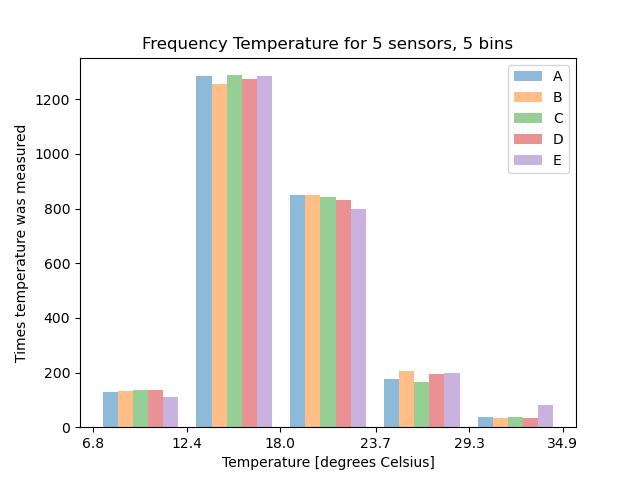
\includegraphics[width=\linewidth]{GEO1001_hw01_images/GEO1001_hw01_A1_hist_5.png}
			\caption{Historgam 5 bins}
		\end{subfigure}
		\begin{subfigure}[b]{0.45\linewidth}
			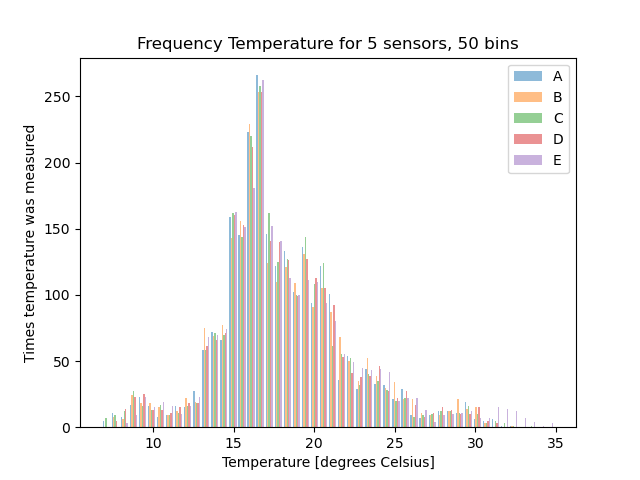
\includegraphics[width=\linewidth]{GEO1001_hw01_images/GEO1001_hw01_A1_hist_50.png}
			\caption{Histogram 50 bins}
		\end{subfigure}
		\caption{Temperature historgam, different nr. of bins}
		\label{fig:histA1}
	\end{figure}

	Figure \ref{fig:histA1} shows the importance of choosing the right number of bins when making a histogram. Both historgams show the distribution of measured temperatures per sensor, but figre b contains a lot more information about the distribution than figure a. A clear peak is indicated, as well as some information about the tails of the distribution and its skewdness. However, figure a does show the differences in distribution between the 5 sensors more clearly. Figure b could be imporved to be less "busy" (e.g. displaying 1 histogram per sensor next to eachother), but as it is right now it is hard to see clear distinctions bewteen sensors.
	
	\subsection{Question 1.3}
	\textbf{Create 1 plot where frequency poligons for the 5 sensors Temperature values overlap in different colors with a legend.}
	
	\begin{figure}[h!]
		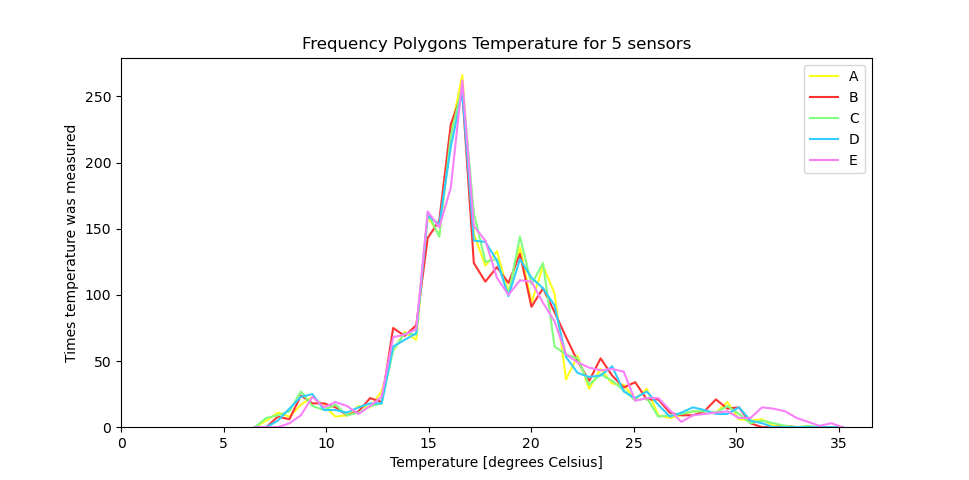
\includegraphics[width=\linewidth]{GEO1001_hw01_images/GEO1001_hw01_A1_polygons.png}
		\caption{Frequency polygons per sensor, Temperature}
		\label{fig:freqpols}
	\end{figure}

	From Firgue \ref{fig:freqpols} it is again visible that the Temperature meansurements for the 5 sensors follow roughtly the same distribution. Sensor E measured higher temperatures, visible in a shorter "left tail" and longer "right tail". All sensors peaks lie around 17 degrees Celsius, this is also where their means will roughly be located.
	
	The figure was made by using the pyplot histogram function. The bins (x-values) were converted into an array of midpoints between all the bin edge points, so each middle point of the histogram bins would correspond to one x-value of the frequency polygon. At the beginning and end of this array, at a distance corresponding with the rest of the series, two zeroes were added, so the polygons would meet the x-axis. Hight values were then interpolated using the histogram values before, and plotted as a line with pyplot. The alpha value of the histograms was set to 0, so only the frequency polygons would be visible in the final plot. The number of bins was determined by simply using pyplots 'auto' parameter, this gave a clear enough image no modifications seemed necessary. The ticks of the x-axis had to be manually set, since using the midpoints themselves resulted in too many x-values to be legible.
	
	
	\subsection{Question 1.4}
	\textbf{Generate 3 plots that include the 5 sensors boxplot for: Wind Speed, Wind Direction and Temperature.}
	
	
	\begin{figure}[H]
		\centering
		\begin{subfigure}[b]{0.7\linewidth}
			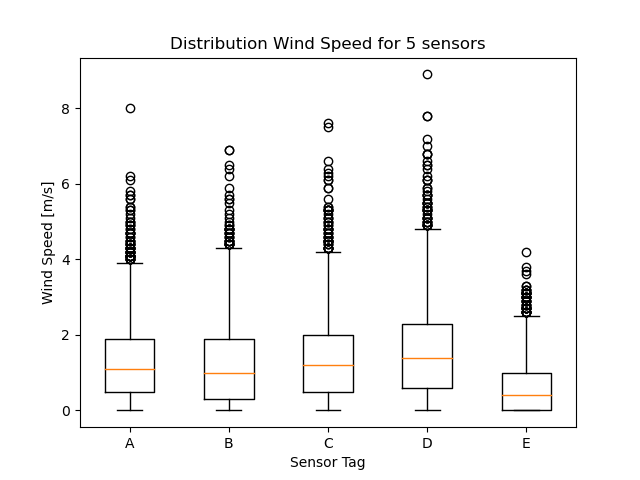
\includegraphics[width=\linewidth]{GEO1001_hw01_images/GEO1001_hw01_A1_box_wind.png}
			\caption{Boxplots 5 sensors, Wind Speed}
			\label{fig:boxwind}
		\end{subfigure}
	
		\begin{subfigure}[b]{0.7\linewidth}
			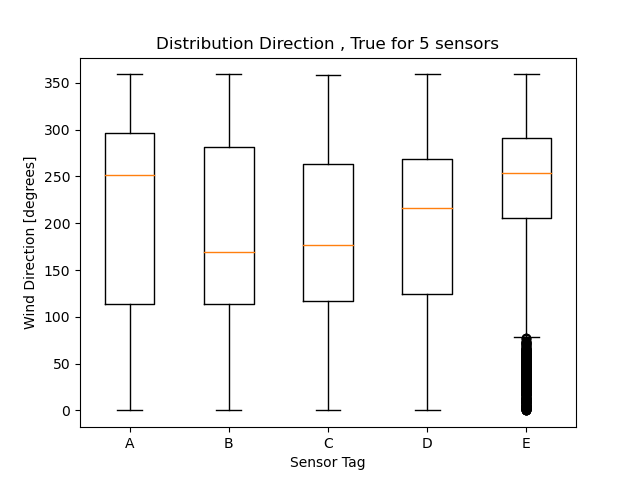
\includegraphics[width=\linewidth]{GEO1001_hw01_images/GEO1001_hw01_A1_box_direction.png}
			\caption{Boxplots 5 sensors, Wind Direction}
			\label{fig:boxdir}
		\end{subfigure}
		
		\begin{subfigure}[b]{0.7\linewidth}
			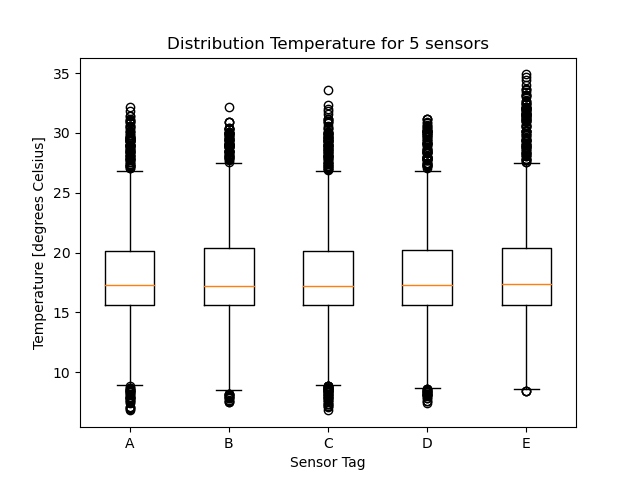
\includegraphics[width=\linewidth]{GEO1001_hw01_images/GEO1001_hw01_A1_box_temp.png}
			\caption{Boxplots 5 sensors, Temperature}
			\label{fig:boxtemp}
		\end{subfigure}
	\end{figure}

	From the Wind Speed boxplot, it can be seen that this variable was measured significantly lower for sensor E. Its minimum value is also barely visible, and it's overal range is also significantly lower than the rest of the sensors. Sensor A to D seem to have about the same interquantile range, with medians also at about the same location. Sensor D has a slightly higher median, IQR, and maximum. All minima are at 0: the sensors may have measured a number of times when there was very little wind. All sensors have many outliers at the top. A possible explaination could be that they have measured a number of high speed wind "bursts", which seems plausible wind behavior.
	
	Figure \ref{fig:boxdir} shows a larger difference between sensors. Maxima and minima are at the same values, except for sensor E. The other sensors measured wind from all directions between their minumum and maximum. Sensor E has many outliers below its minimum: it measured wind from the E/NE direction sometimes, but rarely. There might be a blockade in this direction at sensor E's location, and/or it might have only measured wind from this direction when there was a storm. Sensor B and C's median are both at S/SE, while sensor A's is at W/SW, and sensor D's at SW. All sensor's IQR lies between about W and SE, meaning most wind came from this direction. These plots do correspond with the overal measured wind directions in the Netherlands (Figure \ref{fig:winddirnl}, \cite{journalpone}). Interestingly, this also shows the outliers of sensor E in the east/north-east direction.
	
	
	
	\begin{figure}[H]
		\centering
		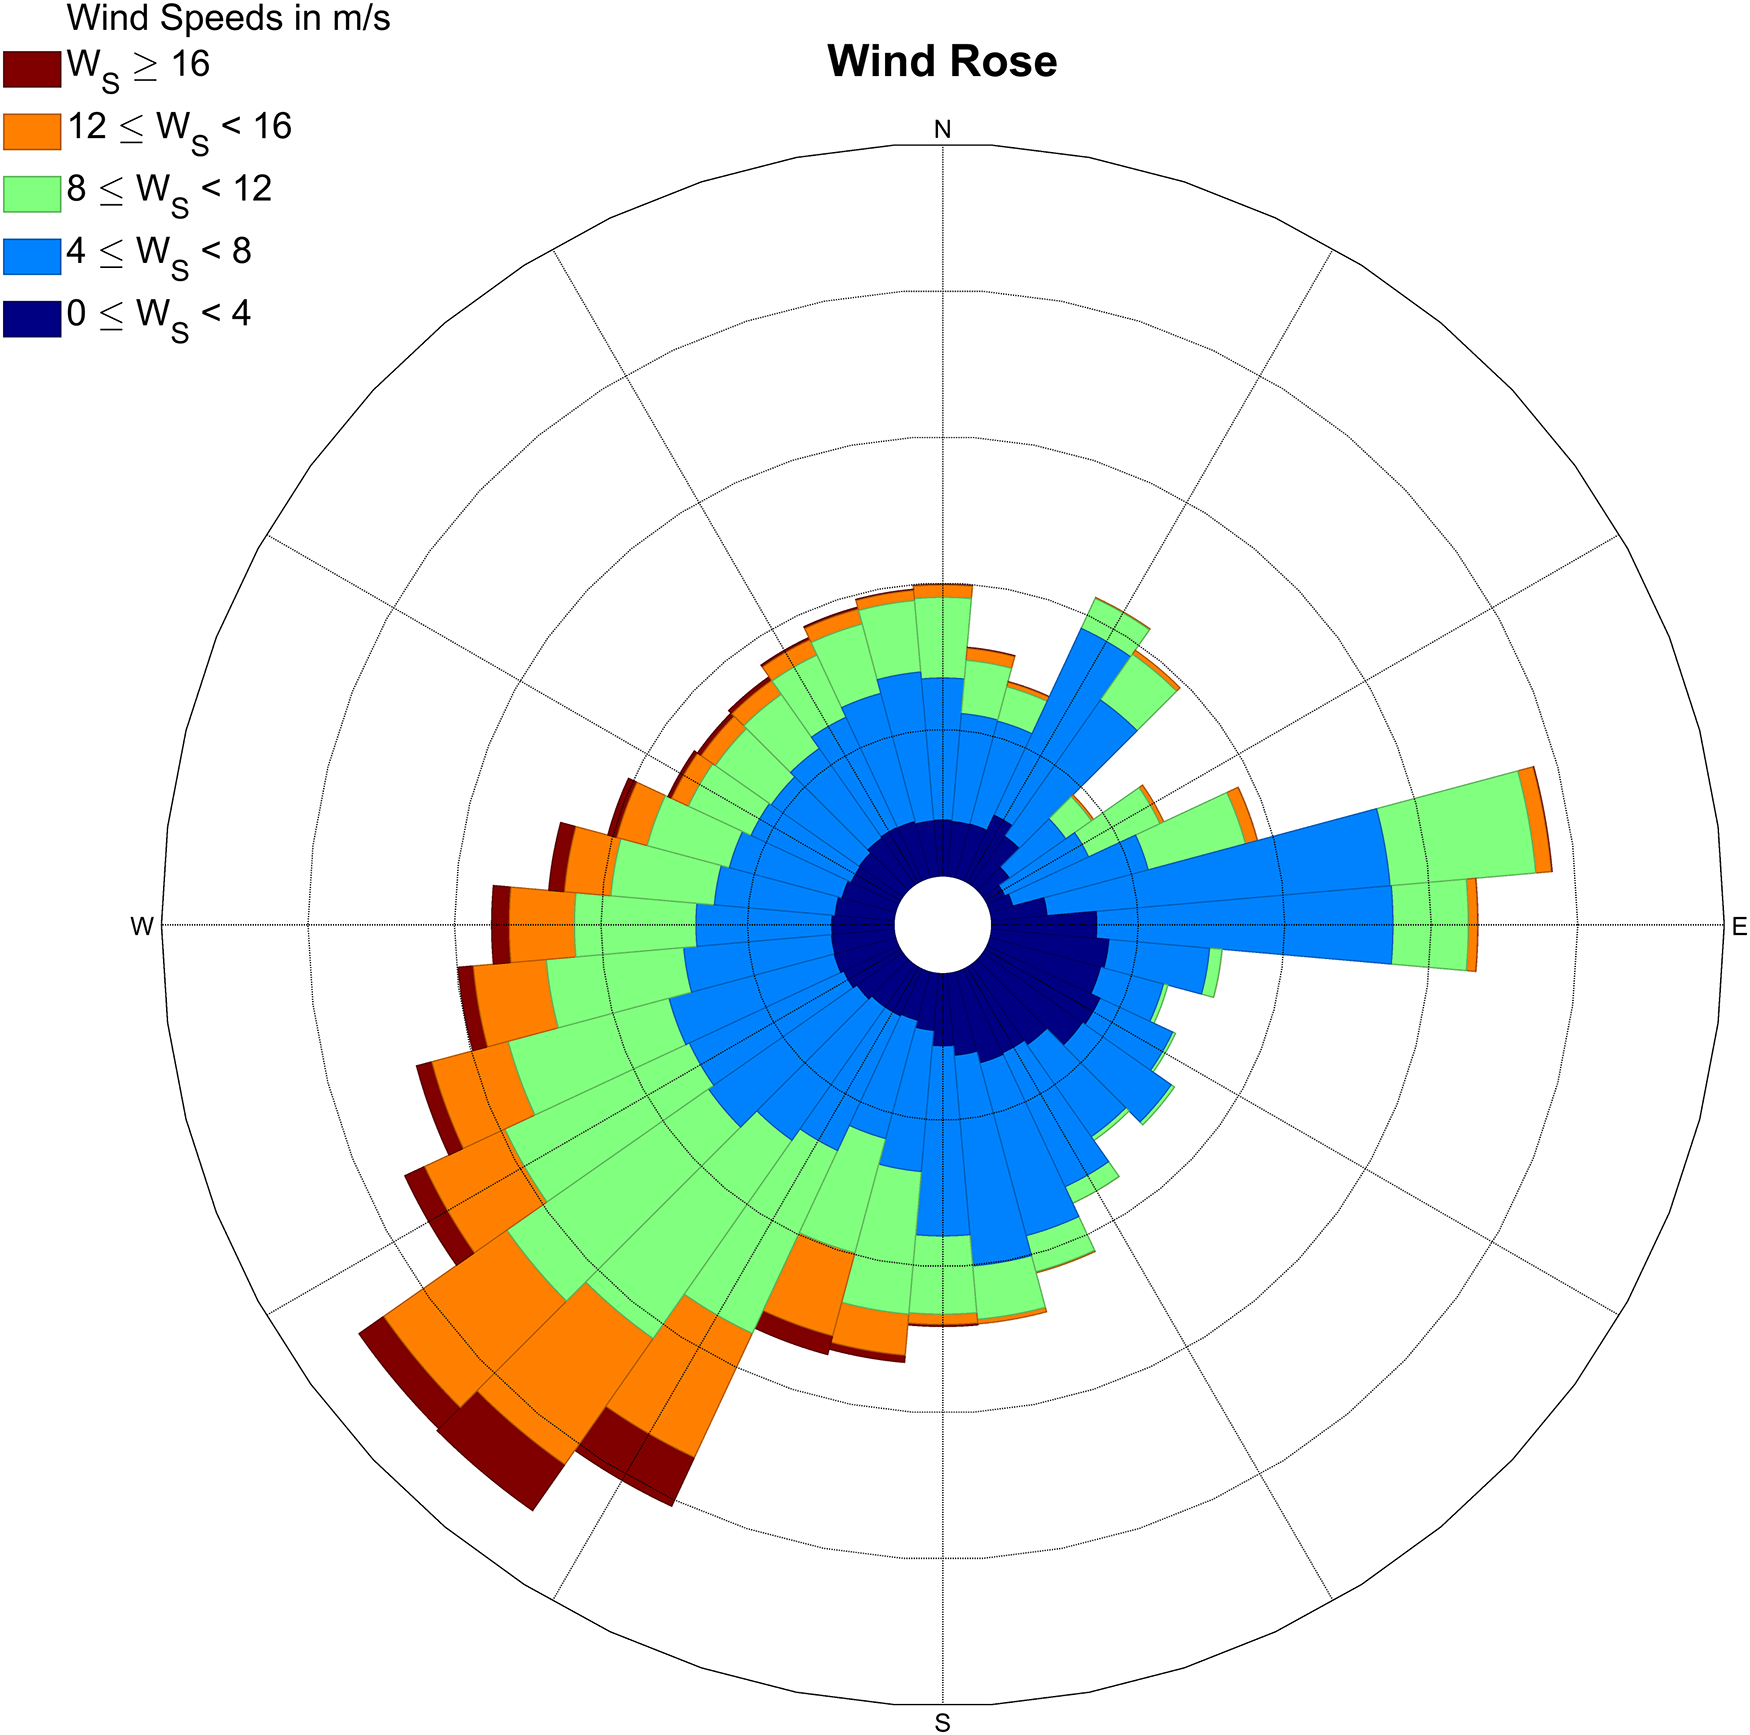
\includegraphics[width=0.7\linewidth]{GEO1001_hw01_images/WindRose_IJmuiden.png}
		\caption{ Wind rose at the IJmuiden weather station based on 10-minute data from January 1, 2007 up to and including December 31, 2016. \cite{journalpone}.}
		\label{fig:winddirnl}
	\end{figure}
	
	\newpage % The first sentence of this paragraph was half displayed on a different page
	The boxplot for Temperature shows little difference between sensors. Sensor E has fewer outliers at the bottom, and more outliers at the highest temperatures. Median and IQR are approximately the same for all sensors. Outliers were detected at the bottom as wel as the top. The measured temperature might only have been very cold and very warm sporadically, showing a moderate climate. Minima seem to be around 7 degrees celsius for all sensors, while maxima are around 27 degrees. Taking into account that measurements were done during the summer, these values seem locical considering the Netherlands's climate.
	
	
	\section{Lesson A2}
	
	\subsection{Question 2.1}
	\textbf{Plot PMF, PDF and CDF for the 5 sensors Temperature values. Describe the behaviour of the distributions, are they all similar? what about their tails?}
	
	 The PMF was made using pyplot's histogram function. The data was first counted per measured temperature (using numpy.value\_counts), normalized and then sorted on increasing temperature values. This resulted in an array with the probability (0 to 1) per measured temperature value per sensor. This was then plotted as a bar plot.
	
	Except for higher values on the y-axis, the PDF shows the same as the PMF. This is because the PDF was made using pyplots histogram, with density set to true. Using the same amount of bins, this will result in the same shape as the PMF. The higher values on the x-axis are a characteristic of the PDF: instead of probability mass, these are the probability densities, meaning the area under the PDF will add up to 1 (instead of all the bar's probabilities itself).
	
	The CDF was done in the same way as the PDF, now with the historgam parameter cumulative also set to true. This results in a bar diagram, where each bar represents the probability of a value in that range, or less, occuring.
	
	From Question 1 it was clear that sensor E measured higher temperatures than the other sensors. The same distribution as the histograms and density polygons can be seen in the PMF and PDF (Figure \ref{fig:pmf}, \ref{fig:pdf}). The lower and upper tails seem to all have their own "local" peaks. The upper tail also seems to be generally longer than the lower for all sensor. This might be a result of measuring the temperature in the summer, when high values are more likely to occur. The effect is also visible in the CDF, where the lower tail of the curve is steeper than the upper tail. 
	
	\newpage
	There also seems to be a slight "bump" in the lower tail of the CDF, corresponding with the local peaks in the PMF and PDF. The Temperature variable's probability funcitons look similar to the shapes of the PMF, PDF and CDF of a normal distribution. The peak, or mean, is slightly more to the left then would be expected. This is visible in the CDF as a smaller incline around this area. Why there would be local peaks in the tails is unclear to me. I speculate this might be a characteristic of complicated wheather phenomena, where low or high temperatures in summer only occur under specific special conditions.
	
	
	\begin{figure}[H]
		\centering
		\begin{subfigure}[b]{\linewidth}
			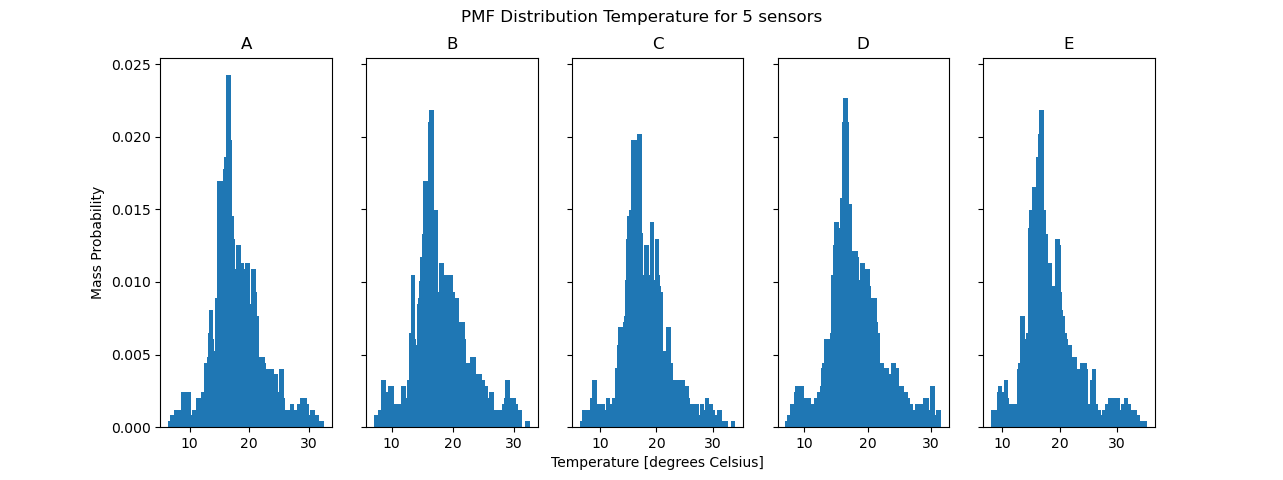
\includegraphics[width=\linewidth]{GEO1001_hw01_images/GEO1001_hw01_A2_PMF.png}
			\caption{Probability mass function, Temperature, all sensors}
			\label{fig:pmf}
		\end{subfigure}
		
		\begin{subfigure}[b]{\linewidth}
			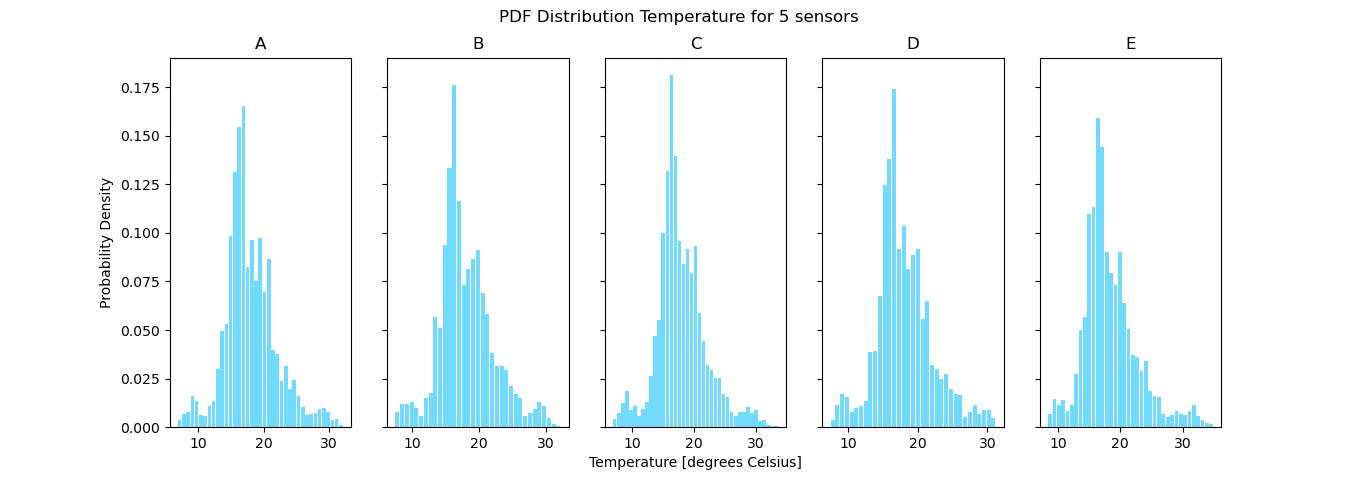
\includegraphics[width=\linewidth]{GEO1001_hw01_images/GEO1001_hw01_A2_PDF.png}
			\caption{Probability density function, Temperature, all sensors}
			\label{fig:pdf}
		\end{subfigure}
		
		\begin{subfigure}[b]{\linewidth}
			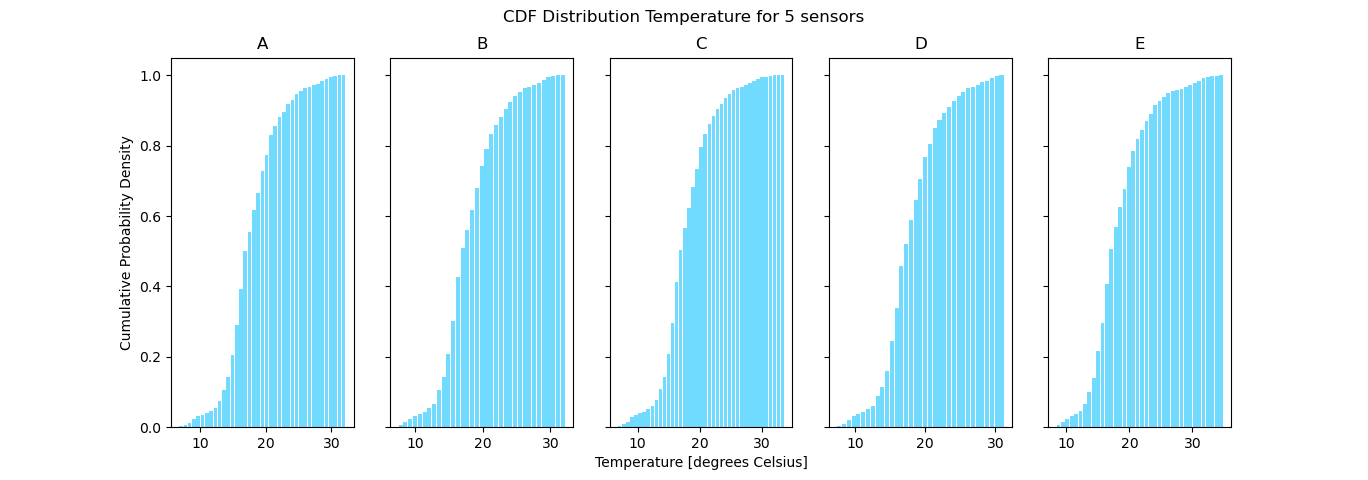
\includegraphics[width=\linewidth]{GEO1001_hw01_images/GEO1001_hw01_A2_CDF.png}
			\caption{Cumulative density function, Temperature, all sensors}
			\label{fig:cdf}
		\end{subfigure}
	\end{figure}
	
	\subsection{Question 2.2}
	\textbf{For the Wind Speed values, plot the pdf and the kernel density estimation. Comment the differences.}
	
	In figure \ref{fig:kde} the PDF of Wind Speed values are combined with the kernel density estimation of it. This figure has the same y-axis, to be able to compare the distributions of all the sensors. Figure \ref{fig:kdeunequal} has an individually scaled y-axis, to better be able to view and compare the shapes of the PDFs and kdes. Sensor E has a very high density around 0, with the PDF even reaching 3. This means that a large amount of the time, this sensor did not measure any wind. In Figure \ref{fig:boxwind}, this was also visible as a significantly lower IQR, maximum, outliers and the minimum and 25th percentile both being on (or around) 0. This sensor is probably located in a more secluded area than the other sensors, where there is less wind. Even though the PDF of the other sensors shows a clear peak, the fitted kde's show 2, where the second one is sometimes even higher than the one corresponding to the PDF peak. The density of the kde at the peak(s) is also much lower than of the PDF. This is a result of the kde being an estimation. It is a funciotn that smoothes the data, and approaches a gaussian function (or what one would expect under a perfect normal distribution). The kde seems to be smooting out the outliers of the funciton, as well as limiting the skewedness.
	
	The kde was first made using pyplot's histogram, with the fitted kde being done by scipy's gaussian estimation. This proved slightly problematic, firstly because it is harder to compare the kde to a bar graph than a line, and secondly because the gaussian kde stopped at x=0, and did not return to the x-axis. The first issue was solved by taking the midpoints of the histogram, like was done for question 1.3, and plotting a line with those values. The second issue, however, seemed to be caused by the way scipy's gaussian kde itself functions. It did not plot any further than the extent of the used dataset, which did stop at 0. It was therefor decided to use seaborn's kde function after all, which had the same shape, but estimated the right tail all the way to the x-axis as well. Both methods are present in the pyhton files for this assignment.
	
	
	\begin{figure}[h!]
		\centering
		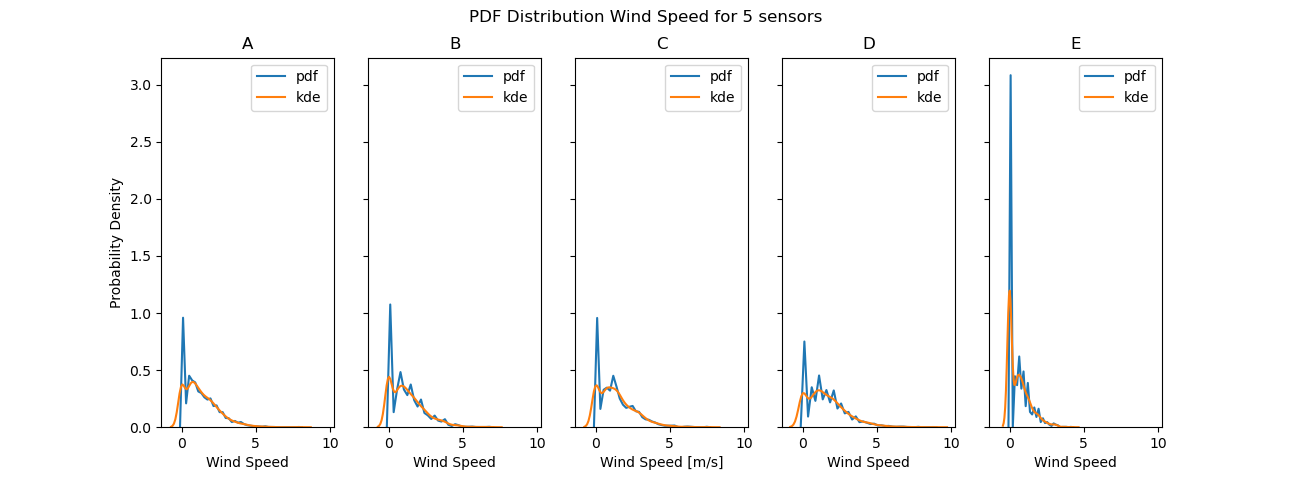
\includegraphics[width=\linewidth]{GEO1001_hw01_images/GEO1001_hw01_A2_kde_compare.png}
		\caption{PDF and kde for all sensors, Temperature}
		\label{fig:kde}
	\end{figure}

	\begin{figure}[h!]
		\centering
		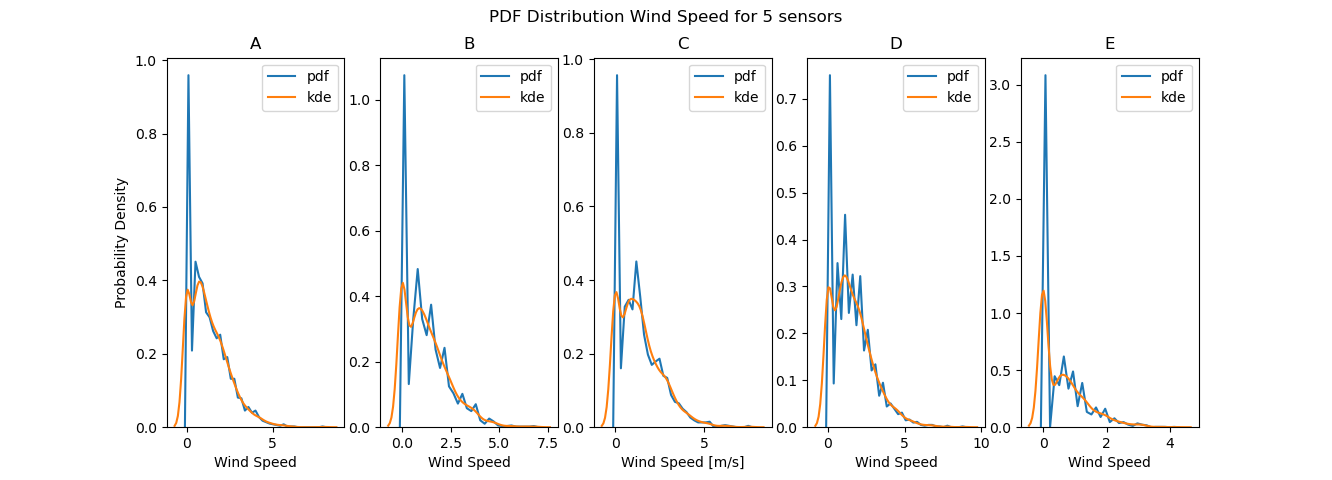
\includegraphics[width=\linewidth]{GEO1001_hw01_images/GEO1001_hw01_A2_kde_original.png}
		\caption{PDF and kde for all sensors, Temperature, unequal scale}
		\label{fig:kdeunequal}
	\end{figure}
	
	\section{Lesson A3}
	
	\subsection{Question 3.1}
	\textbf{Compute the correlations between all the sensors for the variables: Temperature, Wet Bulb Globe, Crosswind Speed. Use Pearson’s and Spearmann’s rank coefficients. Make a scatter plot with both coefficients with the 3 variables.}
	
	\begin{figure}[H]
		\centering
		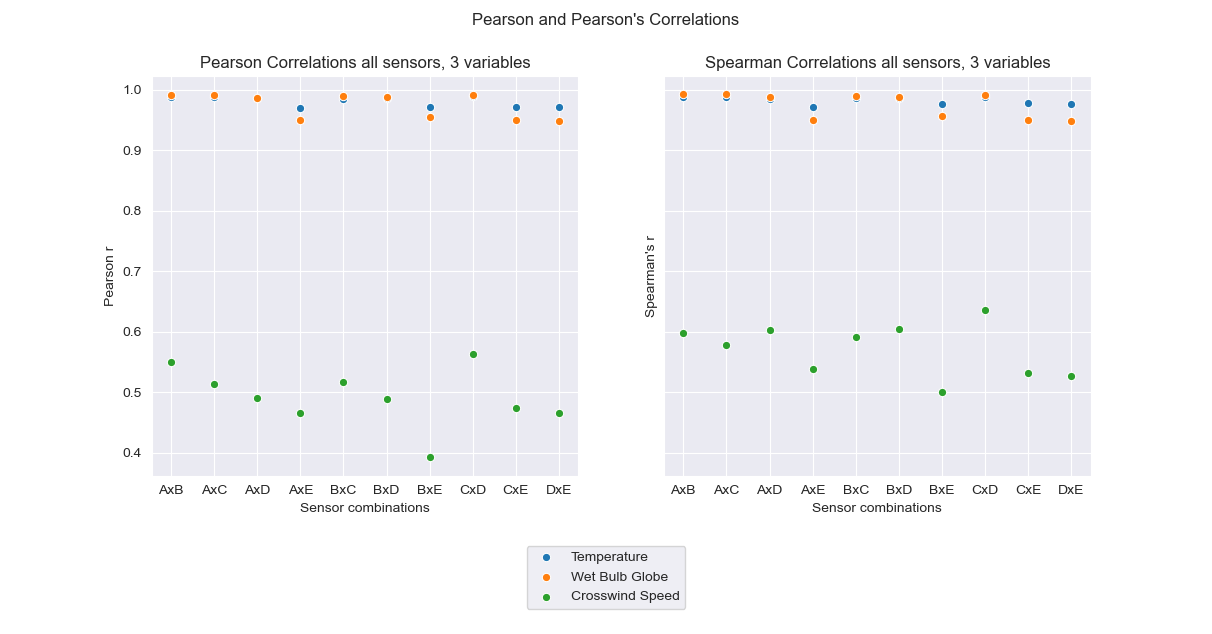
\includegraphics[width=\linewidth]{GEO1001_hw01_images/GEO1001_hw01_A3_correlations.png}
		\caption{correlations between all sensors, Spearman \& Pearson}
		\label{fig:corr}
	\end{figure}
	
	
	\subsection{Question 3.2}
	\textbf{What can you say about the sensors’ correlations?}
	
	Figure \ref{fig:corr} shows sensor E is significantly less correlated with the other sensors: it's Pearson's r and Spearman's $\rho$ are lower for all sensor combinations with sensor E. All Pearson correlation coefficients for Temperature and Wet Bulb Globe Temperature are close to 1, which means there's a very strong positive (linear) correlation between the sensors. The Spearman's rank correlation coefficients are also very close to 1 for these variables. The Pearson's r for Crosswind Speed is significantly lower, lying around 0.5, meaning there's a less strong, but still measurable, correlation between the sensors for this variable. The Spearman's $\rho$ is a bit higher, around 0.6, meaning the colleraltion for Crosswind Speed is not (completely) linear.
	
	\subsection{Question 3.3}
	\textbf{If we told you that that the sensors are located as follows, hypothesize which location would you assign to each sensor and reason your hypothesis using the correlations.}
	
	From Figure \ref{fig:corr}, it is immediately clear that sensor E correlates significantly less with the other sensors. It is therefor likely this sensor is located in the most different spot: the secluded spot at the top. The rest of the locations are less easy to decipher. Differences bewteen correlations are very small. Possible differences could include direction of open spaces around the sensor, terrain type below the sensor, and cover provided by nearby structures. These characteristics are listed in Table \ref{tab:locations}. Locations 1 to 4 are numbered according to Figure \ref{fig:locations}, excluding the location likely to be sensor E. Directions were determined using the top of the image as an (arbitary) north. 
	
	\FloatBarrier
	% Table generated by Excel2LaTeX from sheet 'CI'
	\begin{table}[htbp]
		\centering
		\caption{Possible causes of differences between sensors}
		\resizebox{\textwidth}{!}{\begin{tabular}{lllll}
				\textbf{Location} & \textbf{Dir. open spaces} & \textbf{Dir. cover} & \textbf{Terrain type} & \textbf{Likely sensor} \\
				1     & N   & E, S, W  & field  &C  \\
				2     & N, NE   & E, S, W  & tiles  &D  \\
				3     & N, E  & S, W  & field  &A  \\
				4     & N, S   & E, W  & grassy field  &B  \\	
		\end{tabular}}%
		\label{tab:locations}%
	\end{table}%
	\FloatBarrier
	
	Looking closely at the correlations, it would seem sensor D correlates the least with the other sensors (excluding E).This could be the sensor located on the pavement, which would account for higher measured Temperature and Wet Bulb Globe values. For Crosswind Speed, there seem to be two pairs of sensors which relatively correlate more: A \& B and C \& D. These pairs could be combined with the pairs 1 \& 2 and 3 \& 4 of the sensor locations, which would have the most cmoparable wind speed value pairs. Since C is paired with D, location 1 could correspond to it. The choice of where to place A and B was based on the fact that A correlates a slight bit more with C then B does with C. Location 1 and 3 have the same type of grass, while location 4 has a more lush terrain. This could be a factor in the difference in correlation of sensor A and B with the other sensors. These locations are based on hypotheses, they are not decided with absolute certainty.
	
	The result of the analysis is displayed in Figure \ref{fig:locations}.
	
	\begin{figure}[H]
		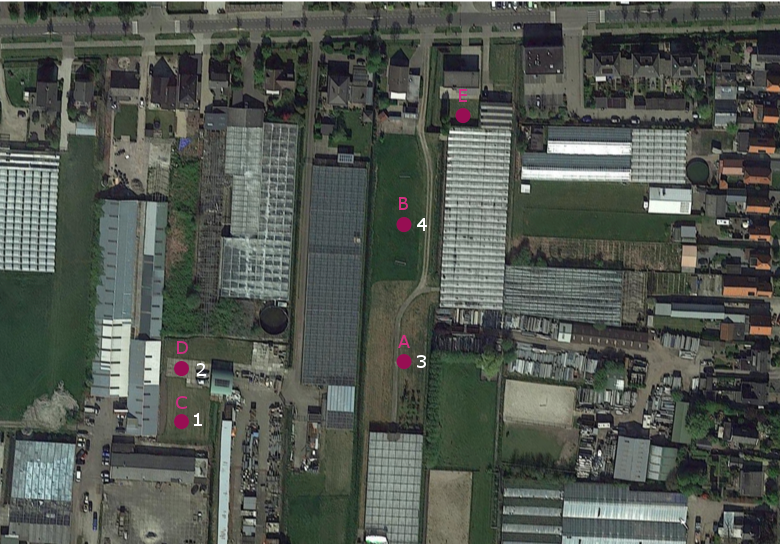
\includegraphics[width=\linewidth]{GEO1001_hw01_images/SensorsSketch_guess.png}
		\caption{Hypothesized locations of sensors}
		\label{fig:locations}
	\end{figure}
	
	
	\section{Lesson A4}
	
	\subsection{Question 4.1}
	\textbf{Plot the CDF for all the sensors and all the variables, then compute the 95\% confidence intervals for all the variables and sensors and save them in a table (txt or csv form).}
	
	Table \ref{tab:ci} shows the confidence intervals calculated from the plotted CDFs (Figure \ref{fig:a4cdf}). The temperature values were determined by finding the x-value for y-values 0.025 and 0.975 on the CDF, since these would correspond to the lower and upper 2,5\% of the symmetrical CDF, leaving 95\% of the values. The means for each sensor are also added to Table \ref{tab:ci}. The confidence intervals do not lie perfectly symmetrical around these means, as one might expect. This is because the interval was extrapolated from a real-life sample, instead of a theoretical distribution function (like a normal distribution). Looking at the shape of the CDF of the Wind Speeds, it would seem likely this variable follows an exponential distribution (as opposed to the (expected) normal distribution of the Temperature).
	
	\begin{figure}[H]
		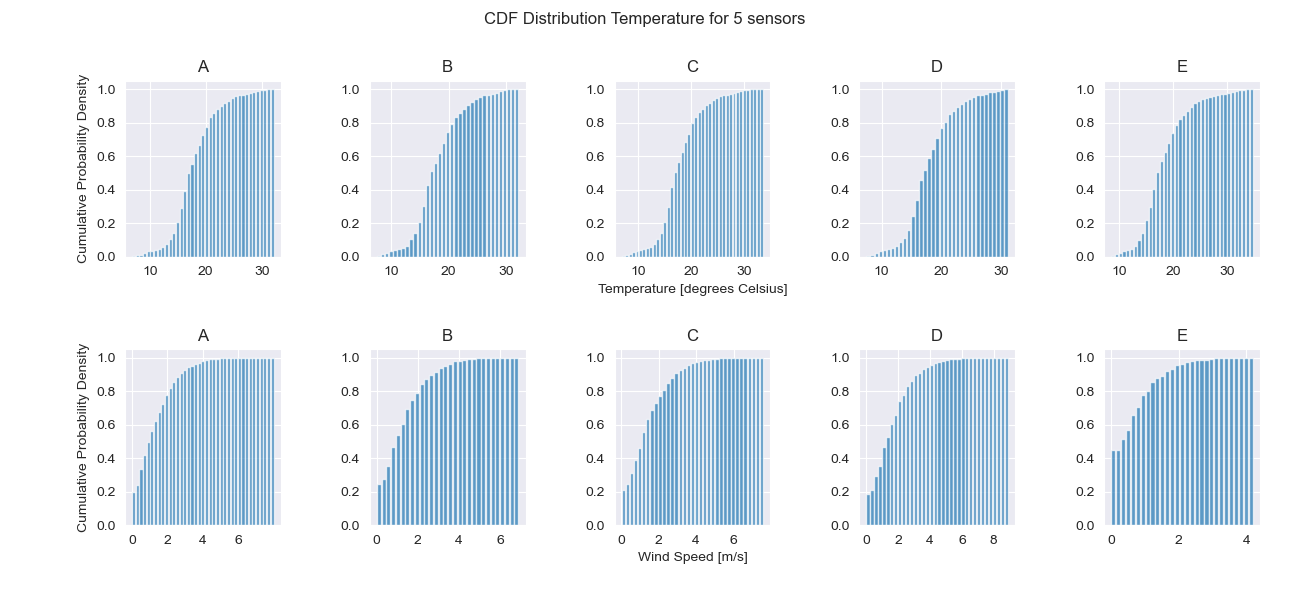
\includegraphics[width=\linewidth]{GEO1001_hw01_images/GEO1001_hw01_A4_CDF.png}
		\caption{Visualisation CDF of all sensors, Temperature \& Wind Speed}
		\label{fig:a4cdf}
	\end{figure}

	\FloatBarrier
	% Table generated by Excel2LaTeX from sheet 'CI'
	\begin{table}[htbp]
		\centering
		\caption{Confidence Interval with mean, Temperature \& Wind Speed}
		\resizebox{\textwidth}{!}{\begin{tabular}{lllllll}
			\textbf{Sensor} & \textbf{CI min Temperature} & \textbf{mean Temperature} & \textbf{CI max Temperature} & \textbf{CI min Wind Speed} & \textbf{mean Wind Speed} & \textbf{CI max Wind Speed} \\
			A     & 9.6   & 18.0  & 28.1  & 0.0   & 1.3   & 4.1 \\
			B     & 9.8   & 18.1  & 28.4  & 0.0   & 1.2   & 3.9 \\
			C     & 9.3   & 17.9  & 28.2  & 0.0   & 1.4   & 4.2 \\
			D     & 9.6   & 18.0  & 27.9  & 0.0   & 1.6   & 4.7 \\
			E     & 10.6  & 18.4  & 30.5  & 0.0   & 0.6   & 2.4 \\
		\end{tabular}}%
		\label{tab:ci}%
	\end{table}%
	\FloatBarrier
	
	
	\subsection{Question 4.2}
	\textbf{Test the hypothesis: the time series for Temperature and Wind Speed are the same for sensors:
	\begin{itemize}
		\item 1) E, D;
		\item 2) D, C;
		\item 3) C, B;
		\item 4) B, A.
	\end{itemize}	}
	
	\FloatBarrier
	% Table generated by Excel2LaTeX from sheet 'Sheet8'
	\begin{table}[htbp]
		\centering
		\caption{t and p values for tested hypotheses}
		\resizebox{\textwidth}{!}{\begin{tabular}{lllll}
			\textbf{sensors} & \textbf{Temperature t} & \textbf{Temperature p} & \textbf{Wind Speed t} & \textbf{Wind Speed p} \\
			ED    & 2.9985 & 0.0027 & -32.6596 & 0.0 \\
			DC    & 0.7294 & 0.4658 & 5.8712 & 0.0 \\
			CB    & -1.3238 & 0.1856 & 3.9088 & 0.0001 \\
			BA    & 0.8408 & 0.4005 & -1.5006 & 0.1335 \\
		\end{tabular}}%
		\label{tab:ttest}%
	\end{table}%
	\FloatBarrier
	

	\subsection{Question 4.3}
	\textbf{What could you conclude from the p-values?}
	
	The hypothesis testing was done with the following parameters:
	\begin{itemize}
		\item H0: $\mu1 - \mu2 = 0$
		\item H1: $\mu1 - \mu2 > 0$
		\item $\alpha = 0.05$
	\end{itemize}
	If the null hypothesis holds, the time series from both sensors would likely be equal. The p-value resulting from the t-tests done for the previous question describes the probability that the observed difference between the means of the 2 samples is due to chance. If this probability is not significant, i.e. smaller than $\alpha$, it is not likely the difference was caused by chance. This means it is likely the samples are actually different, with 1 or more factors other than chance causing a difference in means. The difference in means for Temperature between sensor D and C for example, is 47\% likely to have been due to chance. Here, the H0 was accepted, since this is significantly larger than the predefined 5\%. The conclusions drawn from the p-values are summarized in table \ref{tab:ttestconc}.
	
	\FloatBarrier
	% Table generated by Excel2LaTeX from sheet 'Sheet8'
	\begin{table}[h!]
		\centering
		\caption{conclusions summarized}
		\resizebox{\textwidth}{!}{\begin{tabular}{lllll}
				\textbf{sensors} & \textbf{Temperature} & \textbf{conclusion} & \textbf{Wind Speed} & \textbf{conclusion} \\
				ED    & 0.0027 $<$ 0.05 & reject H0 & 0.0000 $<$ 0.05 & reject H0 \\
				DC    & 0.4658 $>$ 0.05 & accept H0 & 0.0000 $<$ 0.05 & reject H0 \\
				CB    & 0.1856 $>$ 0.05 & reject H0 & 0.0001 $<$ 0.05 & reject H0 \\
				BA    & 0.4005 $>$ 0.05 & accept H0 & 0.1335 $>$ 0.05 & accept H0 \\
		\end{tabular}}%
		\label{tab:ttestconc}%
	\end{table}%
	\FloatBarrier
	
	\newpage
	\bibliography{GEO1001_hw01_bibliography}


	
\end{document}

	